\documentclass[a4paper]{article}

%% Language and font encodings
\usepackage[english]{babel}
\usepackage[utf8x]{inputenc}
\usepackage[T1]{fontenc}
\usepackage{fancyhdr}
\usepackage[at]{easylist}
\usepackage{mathptmx}
\usepackage{bm}
\usepackage{float}
\usepackage{subcaption}
\usepackage{listings}
\usepackage{courier}
\usepackage{siunitx}
\usepackage{framed}
\usepackage{multicol}

\usepackage[bottom]{footmisc}

%% Sets page size and margins
\usepackage[a4paper,top=3cm,bottom=2cm,left=3cm,right=3cm,marginparwidth=1.75cm]{geometry}
\setlength{\parindent}{0pt}

%% Set sections to 1.a etc
\renewcommand{\thesubsection}{\thesection.\alph{subsection}}

%% Useful packages
\usepackage{amsmath}
\usepackage{amssymb}
\usepackage{graphicx}
\usepackage[colorinlistoftodos]{todonotes}
\usepackage[colorlinks=false, allcolors=black]{hyperref}
\usepackage{algpseudocode}
\usepackage{amsmath}
\usepackage{amsfonts}
\usepackage{amssymb}
\usepackage{mathtools}
\usepackage{xcolor}
\definecolor{NAVY}{rgb}{0.2,0.2,1}
\definecolor{YELLOW}{rgb}{1,0.8,0}
\definecolor{LIME}{rgb}{0.5,0.8,0}
\DeclarePairedDelimiter{\ceil}{\lceil}{\rceil}

\title{ENGSCI 355 Project 1}
\author{Logan Wu\\Andrew Jackson\\Scott Sung}
\makeatletter

\setlength{\parskip}{\baselineskip}
\fancyhead{}
\fancyhead[L]{\@title}
\fancyhead[R]{Wu, Jackson, Sung}
\newlength{\drop}
\begin{document}
\begin{titlepage}
    \drop=0.1\textheight
    \centering
    \vspace*{\baselineskip}
    \rule{\textwidth}{1.6pt}\vspace*{-\baselineskip}\vspace*{2pt}
    \rule{\textwidth}{0.4pt}\\[\baselineskip]
    {\LARGE \@title}\\[0.2\baselineskip]
    \rule{\textwidth}{0.4pt}\vspace*{-\baselineskip}\vspace{3.2pt}
    \rule{\textwidth}{1.6pt}\\[\baselineskip]
    \vspace*{2\baselineskip}
    {\Large \textsc{\@author}\par}
    {\itshape Department of Engineering Science\par}
    \vspace*{2\baselineskip}
    {\scshape \today} \        {\large The University of Auckland}\par
    \vspace{\fill}
    \begin{abstract}
    In this report, we describe the mixed-integer formulation to balance patient numbers at a hospital by rostering the registrars in each ward. We predict the infinite-horizon mean occupancies of each ward assuming a Poisson distribution of discharges.
    
We estimate that our program can reduce the average daily imbalance (the difference in patients between the most and least occupied wards each day) by approximately 23\% compared to a random, unoptimised roster. A pairwise analysis of the results reveals that even in the scenario where registrars cannot change their starting weeks, the optimisation program is still able to significantly reduce imbalances.
    \end{abstract}
    \vspace{\fill}
\end{titlepage}
\makeatother
\pagestyle{fancy}

\section{Introduction}

This linear program generates feasible rostering solutions with the aim of minimising the mean expected disparity at any given day between the occupancies of the hospital's wards. The program is flexible, easily accommodating different staff arrangements and historical data with small modifications to a data file.

\section{Assumptions}

\subsection{People are Identical}

To calculate the outcome of a roster, we take advantage of symmetry in the problem and take the liberty of adding some when convenient.

We assume that all ward teams act equally and independently, i.e. there is no difference if we swap the Navy and Lime teams. The state of one ward also does not affect the future state of another. Then we assume that all registrars are equal. Both of these are fair assumptions because registrars usually all have the same background and ward teams are separated, and for three wards with two registrars each, reduce the symmetry by $3!\times2!^3$. We can also fix the night shift week, reducing symmetry by 6.

A trickier assumption is that all patients are independent. This allows us to model them with a Poisson distribution where the mean stay is 2.1 days.
\iffalse\footnote{Weiss, A. J. and Elixhauser, A. (2014). \emph{Overview of Hospital Stays in the United States, 2012}.\\Retrieved from \emph{https://www.hcup-us.ahrq.gov/reports/statbriefs/sb180-Hospitalizations-United-States-2012.pdf}}\fi In reality this should be a heavy-tail distribution (if a patient is going to stay for a while, they will be there for a \emph{long} time), but the memoryless property is a convenient approximation.

\subsection{Occupation Numbers are Periodic}

We assume that the mean admission for each day of the week does not change between weeks, so our admissions data is an average of each day from the past 15 weeks.

We also assume that patient numbers are periodic over the six-week roster. This avoids any discontinuities and checks that the hospital is stable, although this is guaranteed anyway by the Poisson discharge model.

\section{Results}
\begin{table}[H]
\centering
\caption{Final optimised roster. The colour codes are the initial starting weeks for each registrar. Notably, each ward has its registrars three weeks apart.}
\label{tab:roster}
\begin{tabular}{r|ccccccc}
Week	&Mon	&Tue	&Wed	&Thu	&Fri	&Sat	&Sun	\\
\hline
{\color{LIME}$\bullet_1$} 1	& O	& O	& O	& O	& O	& A	& A	\\
{\color{NAVY}$\bullet_1$} 2	& P	& O	& O	& A	& P	& X	& X	\\
{\color{YELLOW}$\bullet_1$} 3	& O	& O	& O	& O	& A	& P	& X	\\
{\color{LIME}$\bullet_2$} 4	& A	& P	& A	& P	& O	& X	& X	\\
{\color{NAVY}$\bullet_2$} 5	& O	& O	& O	& O	& N	& N	& N	\\
{\color{YELLOW}$\bullet_2$} 6	& NO	& NA	& NP	& NO	& ZO	& ZX	& ZX	\\
\end{tabular}
\end{table}

By comparing a series of random, unoptimised rosters ($N=15\times 2$, obtained by disabling the objective function and using both Gurobi and CPLEX) with our roster (Table \ref{tab:roster}), we observe a significant improvement in the daily ward imbalances (Figure \ref{fig:comparison}). On a day-to-day basis using a random roster, the most occupied ward will have an average of between 34 and 36 people ($\alpha = 0.05$) more people than the least occupied. After optimisation, this decreased to 27 -- an estimated reduction of 8 people or 23\%.

While investigating the relative effects, we found no evidence against the hypothesis that the 1\&4, 2\&5, 3\&6 week arrangement was not better than a random arrangement. However, a pairwise analysis before and after adding the objective function (each pair with the same starting week arrangement) found a difference of between 5 and 7 fewer people per day. This shows that even when we cannot optimise the starting weeks as we do using complete enumeration, optimisation still provides a significant improvement.

\begin{figure}[h]
    \centering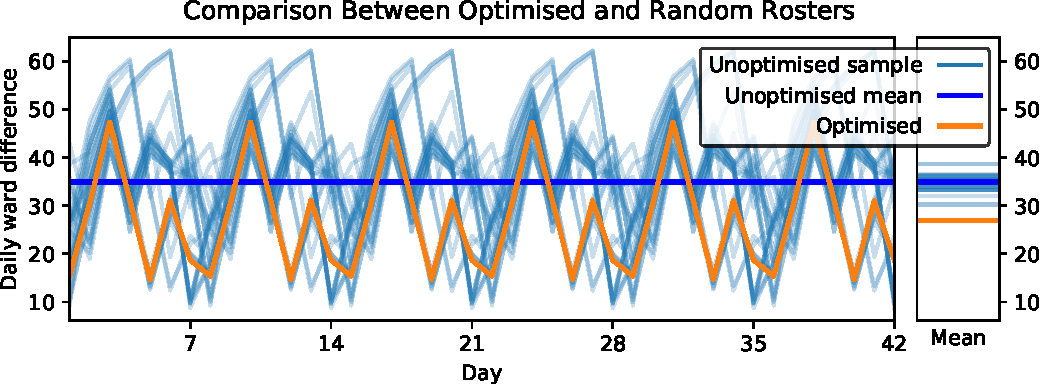
\includegraphics[width=\linewidth]{../results/comparison}
    \caption{Effect of optimisation on day-to-day patient imbalances}
    \label{fig:comparison}
\end{figure}


\section{Conclusion}

Integer programming can drastically reduce hospital ward imbalances compared to a random roster by between 7 and 9 people on average. With more pages, we would display the output from our pairwise analysis of the contributions from different factors (the roster itself vs registrar starting weeks), which concluded that the improvement is mostly due to rearranging the roster shifts, rather than manipulating the relative positioning of each ward's registrars within the roster.

Because we are using predictions for the \emph{expected} patient numbers, our predictions will be resilient to random fluctuations in admissions.

\newpage
\appendix
\section{Formulation}

Our model can be conceptualised as two coupled linear programs. The first is a roster of shifts to ensure feasibility, and the second one is a cyclical network representing ward occupancies during the 42 days of the roster.

\subsection{Parameters}
\begin{multicols}{2}
\noindent


$\mathbb{S} = \{\text{A, P, N, Z, X, O}\}$ \dotfill Set of shift types\\
$\mathbb{W} = \{1, \dots, 6\}$ \dotfill Set of weeks in the roster cycle\\
$\mathbb{D} = \{\text{Mon},\dots,\text{Sun}\}$ \dotfill Set of days in a week\\
$\mathbb{Y}  = \{0, 0,\dots, 0, 1\}$ \dotfill Night shift on the last week

For continuity, a dummy week $0$ and dummy day $\text{Sun}_\text{dummy}$ before Monday also exist but are not part of the sets $\mathbb{W}$ and $\mathbb{D}$. Also, fixing the night shift week takes advantage of symmetry between the weeks.
\end{multicols}
\subsection{Decision Variables}

$X$ is the array of binary variables determining if a type of shift belongs to a given week and day in the roster:
$$x_{s, w, d} \in \{0, 1\} \quad\forall s\in \mathbb{S},\  w\in \mathbb{W} \cup \{0\},\ d\in \mathbb{D} \cup \{\text{Sun}_\text{dummy}\}$$
$V$ denotes whether registrars are forced to take a weekend off:
$$v_w \in \{0, 1\} \quad\forall w\in \mathbb{W} \cup \{\text{Sun}_\text{dummy}\}$$

\subsection{Constraints}

Create a dummy week 0 that is equal to the final week.
\begin{align}
  x_{s, 0, d} = x_{s, |\mathbb{W}|, d} \quad\forall s\in \mathbb{S},\ d\in \mathbb{D}
\end{align}
Create a dummy day 0 that is equal to the last day of the previous week, allowing wrap-around from Sunday to Monday.
\begin{align}
  x_{s, w-1, |\mathbb{D}|} = x_{s, w, 0} \quad\forall s\in \mathbb{S},\ w\in \mathbb{W}
\end{align}
Ensure every slot has a shift assigned by summing over all shift types, except for the night-shift week which must have two.
\begin{align}
  \sum_{s\in \mathbb{S}} x_{s, w, d} - y_w = 1 \quad\forall w\in \mathbb{W},\ d\in \mathbb{D}
\end{align}
Every day must have a single registrar assigned to each A, P and N shift.
\begin{align}
  \sum_{w\in \mathbb{W}} x_{s, w, d} = 1 \quad\forall s\in \{\text{A, P, N}\},\ d\in \mathbb{D}
\end{align}
Every P shift must follow an A shift, except for Sunday where an A must follow an A.
\begin{align}
  x_{\text{P}, w, d} &= x_{\text{A}, w, d-1} \quad\forall w\in \mathbb{W},\ d\in \mathbb{D}\\
  x_{\text{A}, w, d} &= x_{\text{A}, w, d-1} \quad\forall w\in \mathbb{W},\ d\in \{\text{Sun}\}
\end{align}
The Friday to Sunday before the full night shift week are also night shifts.
\begin{align}
  x_{\text{N}, w-1, d} - y_w = 0 \quad\forall w\in \mathbb{W},\ d\in \{\text{Fri, Sat, Sun}\}
\end{align}
The Monday to Thursday of the full night shift week are night shifts.
\begin{align}
  x_{\text{N}, w, d} - y_w = 0 \quad\forall w\in \mathbb{W},\ d\in \{\text{Mon, Tue, Wed, Thu}\}
\end{align}
The Friday to Sunday of the full night shift week are sleep shifts.
\begin{align}
  x_{\text{Z}, w, d} - y_w = 0 \quad\forall w\in \mathbb{W},\ d\in \{\text{Fri, Sat, Sun}\}
\end{align}
Ensure no one else has a sleep shift and is slacking off!
\begin{align}
  \sum_{w\in W,\ d\in \mathbb{D}} x_{\text{Z}, w, d} = 3 \text{ (number of allowed rests)}
\end{align}
No weekdays are allowed to be taken off.
\begin{align}
  x_{\text{X}, w, d} = 0 \quad\forall w\in \mathbb{W},\ d\in \{\text{Mon, \dots, Fri}\}
\end{align}
Weekends must be taken off if scheduled as a 'weekend off' (but may be taken off on other weekends).
\begin{align}
  x_{\text{X}, w, d} \ge 0 \quad\forall w\in \mathbb{W},\ d\in \{\text{Sat, Sun}\}
\end{align}
No two consecutive weekends can pass without a weekend off being forced.
\begin{align}
  v_w + v_{w-1} \ge 1 \quad\forall w\in \mathbb{W}
\end{align}

\subsection{Objective Parameters}

There are several new definitions that are particular to this section of the formulation. This section can be represented as a 42-node cycle with discounted arcs between consecutive nodes, and artificial insertions on admission days averaged from the 15-week data.

\begin{multicols}{2}
\begin{flushright}
$\mathbb{WA} = \{\text{lime},\ \text{navy},\ \text{yellow}\}$ \dotfill Set of wards\\
$\mathbb{R} = \mathbb{W}\times \mathbb{D}$ \dotfill Set of all days in the roster, to simplify $r+1$ and $r-1$ subscripts\\
$\rho = 0.45$ \dotfill Poisson constant for discharges\\
$s_{wa,re}$ \dotfill See following paragraph
\end{flushright}

$s_{wa, re} \in \mathbb{W}$ is an array of unique starting weeks for each registrar in each ward. $s_{wa, re}$ is not a decision variable of the IP; rather, it is a meta-variable, enumerated by a tree with 15 unique combinations.
\end{multicols}
\subsection{Objective-Related Variables}

A is a unimodular matrix determining whether a ward is admitting on a certain day.
$$a_{wa, r} \in \{0,\ 1\} \quad\forall wa\in \mathbb{WA},\ r\in \mathbb{R}$$
O is a matrix of each ward's \emph{expected} occupancy for each day in the roster (we use expectation values to deal with the stochastic nature of ward numbers).
$$o_{wa, r} \ge 0 \quad\forall wa\in \mathbb{WA},\ r\in \mathbb{R}$$
$\dot{\text{P}}$ is the expected daily admission rate for each day of the week.
$$\dot{p_{d}} \in Z^+ \quad\forall d\in \mathbb{D}$$
$\Delta$ is the maximum pairwise difference between all wards for a given day of the roster.
$$\delta_r \ge 0 \quad\forall r \in \mathbb{R}$$

\subsection{Objective Constraints and Objective Function}

These constraints calculate the expected mean occupancy of each ward throughout the 42-day roster. $\%$ is the modulo function and $\ceil{x}$ rounds up to the nearest integer.

Control whether a ward is admitting on a given day of the 6-week cycle. The absolutely insane subscripts adjust for starting week offsets; i.e. on week one, day one, a registrar who started on week six will actually be looking at week six, day one of the roster.
\begin{align}
  a_{wa, (r+1)\%|\mathbb{R}|+1} = \sum_{re\in \{1\dots n_\text{registrars}\}}{x_{\text{A}, \ceil{\frac{r+|\mathbb{D}|\text{s}_{wa, re}-1}{|\mathbb{D}|}} \% |\mathbb{W}|+1, (r-1) \% |\mathbb{D}|+1}} \quad\forall wa \in \mathbb{WA},\ r \in \mathbb{R}
\end{align}
Calculate the expected occupancy based on the discounted occupancy from the previous day, plus the previous day's admissions if the ward was admitting. We used a mean stay of 2.1 days to model discharges as a Poisson process with a rate of 0.45.
\begin{align}
  o_{wa, r\%|\mathbb{R}|+1} = o_{wa, r} \times (1-\rho) + a_{wa, r} \times \dot{p}_{(r-1)\%|\mathbb{D}|+1} \quad\forall wa \in \mathbb{WA},\ r \in \mathbb{R}
\end{align}
For each day calculate the range of ward occupant numbers (the maximum pairwise difference).
\begin{align}
  \delta_r \ge o_{wa, r} - o_{wb, r} \quad\forall r \in \mathbb{R},\ wa \in \mathbb{WA},\ wb \in \mathbb{WA}
\end{align}

\begin{framed}
Objective function: Minimise the range of patient numbers, summing over all days in the roster.
\begin{align}
  \text{minimise} \sum_{r\in \mathbb{R}}{\delta_r}
\end{align}
\end{framed}

\end{document}
